\section{Funcionamento e interfaceamento do CLP}

\begin{frame}{Introdução}
	\begin{block}{}
		\begin{itemize}
			\item Na aula anterior entendemos a \textbf{função do CLP num processo}, além de alguns acessórios \textbf{necessários} para sua operação.
			\item Agora vamos nos aprofundar no seu \textbf{funcionamento}, entendendo como opera.
		\end{itemize}
	\end{block}

	\centering
	
	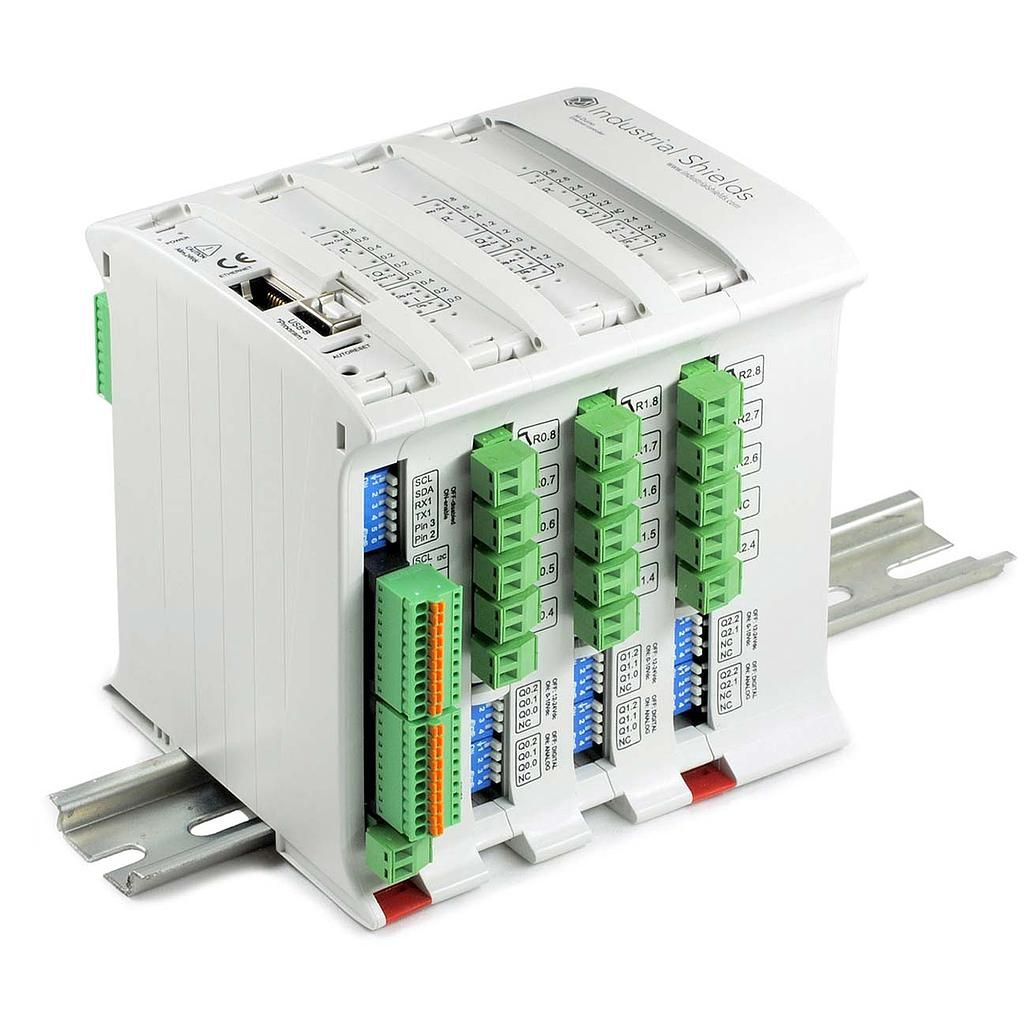
\includegraphics[height=0.6\textheight]{Figuras/Ch09/fig1}
\end{frame}


\begin{frame}{Funcionamento}
	\begin{block}{Varredura}
		O CLP funciona num ciclo chamado de \textbf{varredura}, onde:
		\begin{enumerate}
			\item Realiza a \textbf{leitura das entradas}, através dos seus \textit{Cartões de input};
			\item \textbf{Executa o programa} salvo em sua \textit{Memória de programa};
			\item \textbf{Atualiza as saídas} nos \textit{Cartões de output}.
		\end{enumerate}
	\end{block}
	
	\vspace{0.2cm}
	
	\centering
	
	\begin{tikzpicture}[scale=0.5]
	\draw (-4,-3) rectangle (4,3); %CLP
	\draw (-4,0) -- (-2.5,0); %Div in out
	\draw (-2.5,-3) -- (-2.5,3); %Div cartoes
	\draw (-1.5,-2.5) rectangle (0,2.5); %Mem dados
	\draw (0.5,-2.5) rectangle (3.5,-1); %Mem prog
	\draw (1,0) rectangle (3,2); %CPU
	
	\draw (1,2.6) node {CLP};
	
	\draw (-3.25,1.5) node[text width=1.5cm,align=center,rotate=90] {\small Cartões de input};
	
	\draw (-3.25,-1.5) node[text width=1.5cm,align=center,rotate=90] {\small Cartões de output};
	
	\node at (2,1) {\small CPU};
	
	\node[rotate=90,text width=1.5cm,align=center] at (-0.75,0) {\small Memória de dados};
	
	\node[text width=2cm,align=center] at (2,-1.75) {\footnotesize Memória de programa};
	
	\node at (-6,0) {Campo};
	
	\draw[-Latex] (-8,1.5) -- node[above] {Entradas} +(4,0);
	\draw[Latex-] (-8,-1.5) -- node[below] {Saídas} +(4,0);
	\draw[-Latex] (-2.5,1.5) -- +(1,0);
	\draw[Latex-] (-2.5,-1.5) -- +(1,0);
	\draw[-Latex] (0,1.5) -- +(1,0);
	\draw[Latex-] (0,0.5) -- +(1,0);
	\draw[Latex-] (2,0) -- +(0,-1);
	\end{tikzpicture}
\end{frame}


\begin{frame}{Funcionamento}
	\begin{block}{Cartões}
		\begin{itemize}
			\item Os cartões tem a função de \textbf{interfacear} o CLP com o ambiente externo do chão de fábrica.
			\item Existem 4 tipos de interfaces possíveis:
			\begin{enumerate}
				\item AIs - \textit{Analogue Inputs} (Entradas analógicas)
				\item AOs - \textit{Analogue Outputs} (Saídas Analógicas)
				\item DIs - \textit{Digital Inputs} (Entradas Digitais)
				\item DOs - \textit{Digital Outputs} (Saídas Digitais)
			\end{enumerate}
		\end{itemize}
	\end{block}

	\centering
	
	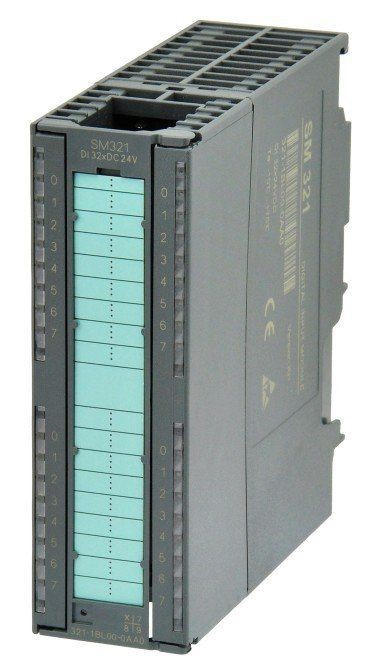
\includegraphics[height=0.4\textheight]{Figuras/Ch09/fig2}
\end{frame}


\begin{frame}{Funcionamento}
	\begin{block}{Cartões}
		\begin{itemize}
			\item As \textbf{entradas} são por onde os dados \textbf{entram} no CLP.
			\item As \textbf{saídas} são por onde os dados \textbf{saem} do CLP.
			\item Sinal \textbf{analógico} é aquele que é \textbf{contínuo} (pode ser \textbf{qualquer valor} - \textbf{entre} 0 e 1, por exemplo).
			\item Sinal \textbf{digital} é aquele que é \textbf{descontínuo} (tem \textbf{valores exatos} - 0 \textbf{ou} 1, por exemplo).
		\end{itemize}
	\end{block}
	
	\begin{minipage}{0.48\linewidth}
		\centering
		
		\scalebox{0.45}{

\tikzset{every picture/.style={line width=0.75pt}} %set default line width to 0.75pt        

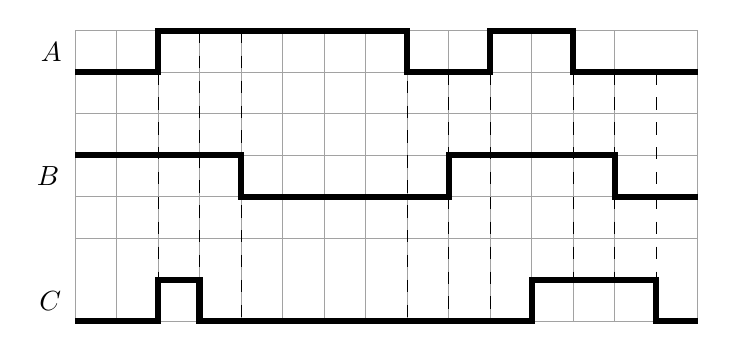
\begin{tikzpicture}[x=0.75pt,y=0.75pt,yscale=-1,xscale=1]
%uncomment if require: \path (0,300); %set diagram left start at 0, and has height of 300

%Shape: Grid [id:dp34531111101152123] 
\draw  [draw opacity=0] (100,40) -- (400,40) -- (400,180) -- (100,180) -- cycle ; \draw  [color={rgb, 255:red, 162; green, 162; blue, 162 }  ,draw opacity=1 ] (120,40) -- (120,180)(140,40) -- (140,180)(160,40) -- (160,180)(180,40) -- (180,180)(200,40) -- (200,180)(220,40) -- (220,180)(240,40) -- (240,180)(260,40) -- (260,180)(280,40) -- (280,180)(300,40) -- (300,180)(320,40) -- (320,180)(340,40) -- (340,180)(360,40) -- (360,180) ; \draw  [color={rgb, 255:red, 162; green, 162; blue, 162 }  ,draw opacity=1 ] (100,60) -- (400,60)(100,80) -- (400,80)(100,100) -- (400,100)(100,120) -- (400,120)(100,140) -- (400,140) ; \draw  [color={rgb, 255:red, 162; green, 162; blue, 162 }  ,draw opacity=1 ] (100,40) -- (400,40) -- (400,180) -- (100,180) -- cycle ;
%Straight Lines [id:da9908667716444586] 
\draw  [dash pattern={on 4.5pt off 4.5pt}]  (140,60) -- (140,160) ;


%Straight Lines [id:da9489034074703155] 
\draw  [dash pattern={on 4.5pt off 4.5pt}]  (160,40) -- (160,160) ;


%Straight Lines [id:da7444148673969375] 
\draw  [dash pattern={on 4.5pt off 4.5pt}]  (180,40) -- (180,180) ;


%Straight Lines [id:da33359589579811755] 
\draw  [dash pattern={on 4.5pt off 4.5pt}]  (260,40) -- (260,180) ;


%Straight Lines [id:da1689198722872045] 
\draw  [dash pattern={on 4.5pt off 4.5pt}]  (280,60) -- (280,180) ;


%Straight Lines [id:da2835936693187402] 
\draw  [dash pattern={on 4.5pt off 4.5pt}]  (300,60) -- (300,180) ;


%Straight Lines [id:da7069604701418795] 
\draw  [dash pattern={on 4.5pt off 4.5pt}]  (340,60) -- (340,160) ;


%Straight Lines [id:da35256438922338873] 
\draw  [dash pattern={on 4.5pt off 4.5pt}]  (360,60) -- (360,160) ;


%Straight Lines [id:da8396949759627998] 
\draw  [dash pattern={on 4.5pt off 4.5pt}]  (380,60) -- (380,160) ;


%Straight Lines [id:da8850959184881091] 
\draw [line width=2.25]    (100,60) -- (140,60) -- (140,40) -- (260,40) -- (260,60) -- (300,60) -- (300,40) -- (340,40) -- (340,60) -- (400,60) ;


%Straight Lines [id:da2574956876601695] 
\draw [line width=2.25]    (100,180) -- (140,180) -- (140,160) -- (160,160) -- (160,180) -- (320,180) -- (320,160) -- (380,160) -- (380,180) -- (400,180) ;


%Straight Lines [id:da8609754683162194] 
\draw [line width=2.25]    (100,100) -- (180,100) -- (180,120) -- (280,120) -- (280,100) -- (360,100) -- (360,120) -- (400,120) ;



% Text Node
\draw (88.5,50) node   {$A$};
% Text Node
\draw (87,110) node   {$B$};
% Text Node
\draw (88,170) node   {$C$};


\end{tikzpicture}
}
		
		Sinal analógico
	\end{minipage}
	\hfill
	\begin{minipage}{0.48\linewidth}
		\centering
		
		\scalebox{0.45}{\deftkzbds
		
\begin{tikzpicture}[auto, node distance=2cm,>=Latex]
	% We start by placing the blocks
	\node [input] (input) {};
	\node [block, right=of input, xshift=0cm, align=center, text width=2cm] (computer) {$ h[n] $};
	\node [output, right =of computer] (output) {};
	\node [above, xshift=0.8cm] at (input) {$ x\left[n \right]  $};
	\node [above, xshift=-1cm] at (output) {$ y\left[n \right]  $};
	
	\draw [->] (input) -- (computer);
	\draw [->] (computer) -- (output);
\end{tikzpicture}}
		
		Sinal digital
	\end{minipage}
\end{frame}


\begin{frame}{Funcionamento}
	\begin{block}{Cartões de entrada}
		Os cartões de entrada devem pegar o \textbf{sinal puro}, geralmente de $ 4 $ a \SI{20}{\milli\ampere}, e \textbf{convertê-lo} para \textbf{binário}, mas \textbf{como} fazem isso?
		\begin{itemize}
			\item Caso o sinal seja \textbf{digital} o cartão irá converter o sinal de \textbf{ativado} (normalmente \SI{20}{\milli\ampere}) para um bit $ 1 $, e o sinal de \textbf{desativado} para um bit $ 0 $.
			\item Caso o sinal seja \textbf{analógico} o cartão pode representá-lo por um conjunto de bits.
		\end{itemize}
	
		Um cartão de saída realiza o processo inverso.
		
		\medskip
	
		\textbf{Obs.:} Via de regra, quanto \textbf{mais bits}, \textbf{mais exata a representação} deste sinal, mas \textbf{nunca} será perfeita.
	\end{block}
\end{frame}


\begin{frame}{Funcionamento}
	\begin{block}{Memórias e cartões}
		\begin{itemize}
			\item Quando um cartão de entrada lê um valor, precisa \textbf{escrevê-lo} em algum lugar, e este lugar é a \textit{memória de dados}.
			\item Essa memória serve como \textbf{área de trabalho} para o CLP, assim como local de \textbf{repassagem de valores} entre os cartões e o controlador.
			\item Depois que o CLP realiza o processamento do \textbf{programa do usuário}, \textbf{devolve os valores alterados} para a memória de dados, de onde os cartões de saída \textbf{lerão o novo valor} para ser passado para o processo, e vão \textbf{atualizar seu estado}.
			\item Isso é o \textbf{ciclo de varredura}.
		\end{itemize}
	\end{block}
\end{frame}


\begin{frame}{Funcionamento}
	\begin{block}{Memórias}
		\begin{itemize}
			\item O CLP possui duas memórias \textbf{distintas}.
			\item A \textit{memória de dados} é a de \textbf{uso comum} do CLP, e pode ser \textbf{escrita} e \textbf{acessada} por ele.
			\item A \textit{memória de programa} é responsável por \textbf{guardar} o programa do usuário dentro do CLP, ela pode ser \textbf{acessada}, mas \textbf{não} alterada por ele.
			\item Essa distinção é importante para que não se \textbf{comprometa} o programa do usuário de \textbf{nenhuma forma}.
		\end{itemize}
	\end{block}
\end{frame}


\begin{frame}{Funcionamento}
	\begin{block}{Modos de operação}
		De maneira geral, o CLP pode estar em dois estados:
		\begin{itemize}
			\item Modo \textbf{RUN}, onde o CLP funcionará normalmente, executando o programa carregado.
			\item Modo \textbf{PROG}, onde o CLP estará inativo, aguardando o \textbf{download} de um novo programa.
		\end{itemize}
		Quando o CLP é programado durante seu funcionamento, chamamos isso de programação \textbf{online}, e quando programamos ele no modo \textbf{PROG}, isso é chamado de programação \textbf{offline}.
		
		\medskip
		
		\textbf{Obs.:} O CLP também pode entrar em \textbf{modo de falha}, caso ocorra algum problema na execução do programa do usuário, e isso às vezes é considerado um possível estado, assim como o estado \textbf{STOP}, no qual o CLP está desligado, ou, inativo.
	\end{block}
\end{frame}


\begin{frame}{Funcionamento}
	\begin{block}{Inicialização}
		\begin{itemize}
			\item A cada inicialização de um novo loop, o CLP executa um teste automático para verificar o funcionamento de todo seu circuito interno.
			\item Caso haja alguma falha ou alguma anormalidade em seu sistema (falha na memória ou no	processador, por exemplo) um sinal de alarme é enviado para avisar o operador.
			\item Isso é chamado de \textbf{``teste de circuito interno''}.
			\item O CLP também protege suas memórias em situações em que ocorra a falta de energia, alimentando-as automaticamente pelo sistema através das baterias de backup, de modo a evitar a perda de dados.
		\end{itemize}
	\end{block}
\end{frame}


\begin{frame}{Funcionamento}
	\begin{block}{Tipos de tarefas}
		Existem três tipos de tarefas num CLP:
		\begin{itemize}
			\item Tarefas \textbf{contínuas}, que devem ser executadas a todo momento.
			\item Tarefas \textbf{de tempo}, que devem ser executadas em intervalos exatos.
			\item Tarefas \textbf{de eventos}, que devem ser executadas em situações específicas (erro, por exemplo).
		\end{itemize}
	\end{block}
\end{frame}


\begin{frame}{Funcionamento}
	\begin{block}{Tipos de tarefas}
		Para ilustrar os tipos de tarefas, podemos pensar no exemplo de uma \textbf{máquina de estampar} numa \textbf{linha de produção}:
	\end{block}

	\centering
	
	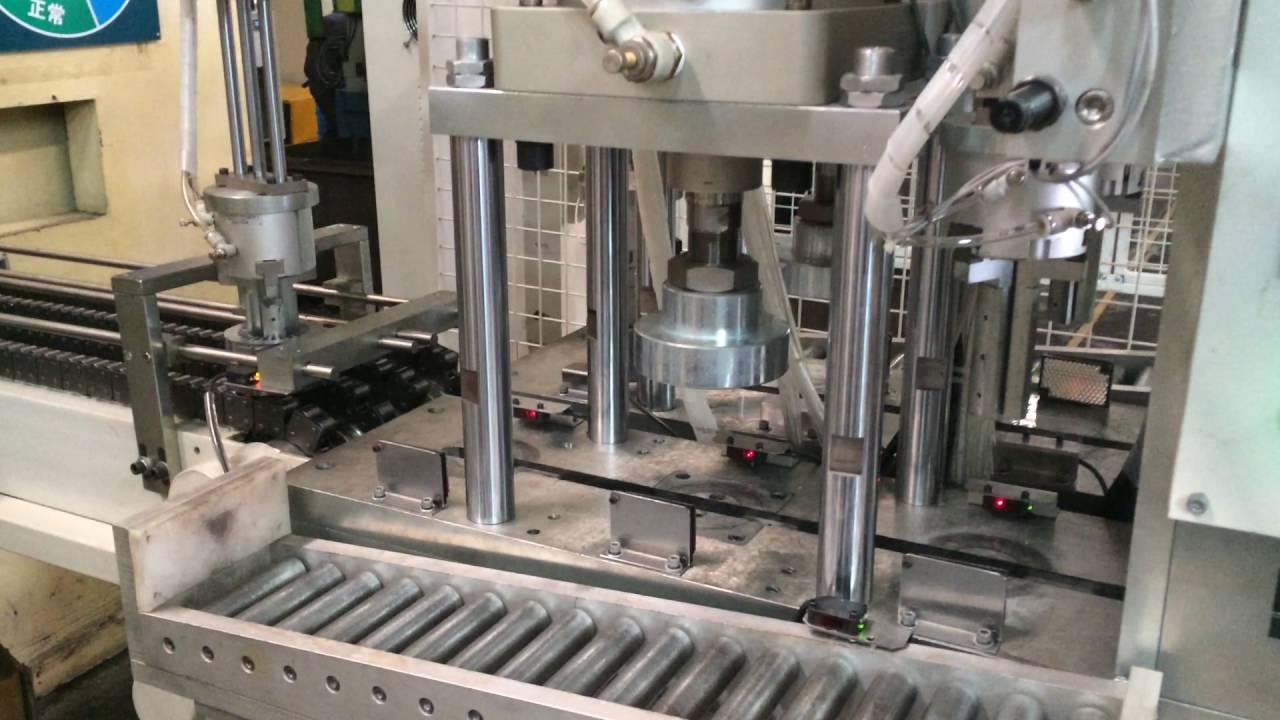
\includegraphics[height=0.6\textheight]{Figuras/Ch09/fig3}
\end{frame}


\begin{frame}{Funcionamento}
	\begin{block}{Tipos de tarefas}
		\begin{itemize}
			\item A esteira deve permanecer em movimento \textbf{constantemente} -- \textit{tarefa contínua}.
		\end{itemize}
	\end{block}
	
	\centering
	
	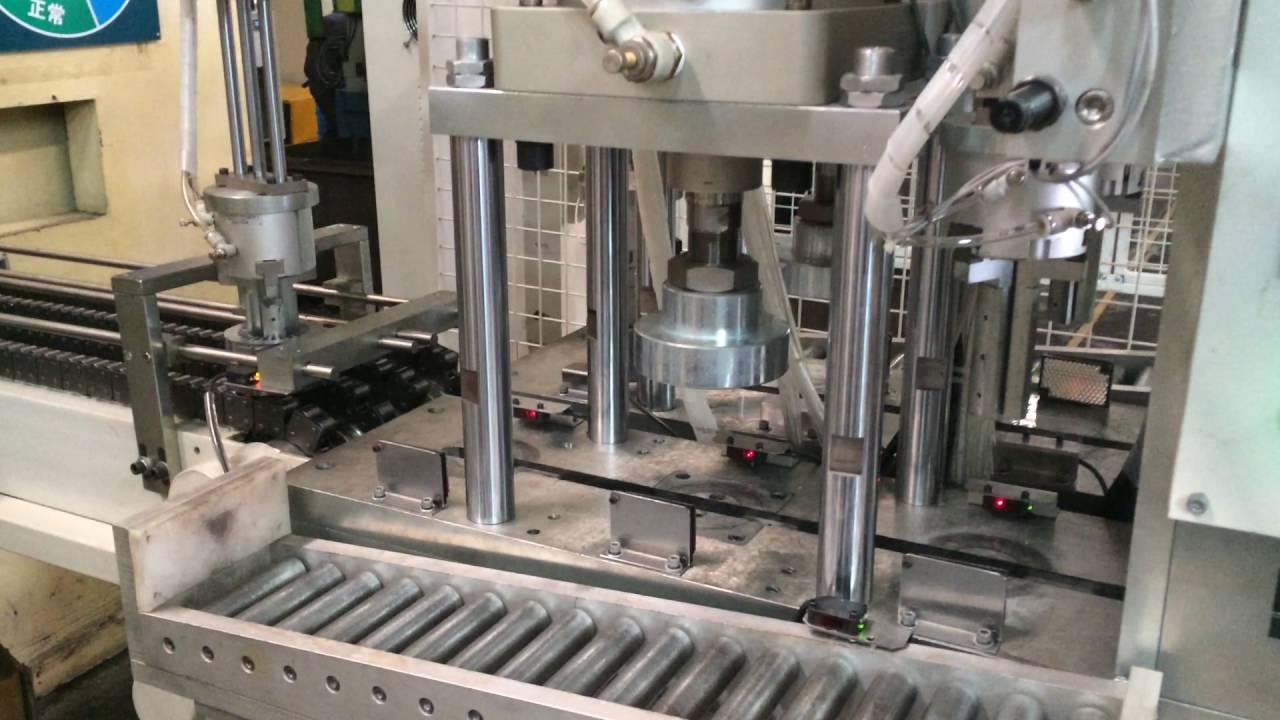
\includegraphics[height=0.6\textheight]{Figuras/Ch09/fig3}
\end{frame}


\begin{frame}{Funcionamento}
	\begin{block}{Tipos de tarefas}
		\begin{itemize}
			\item A máquina de estampar deve aplicar uma nova estampa \textbf{em intervalos} regulares -- \textit{tarefa de tempo}.
		\end{itemize}
	\end{block}
	
	\centering
	
	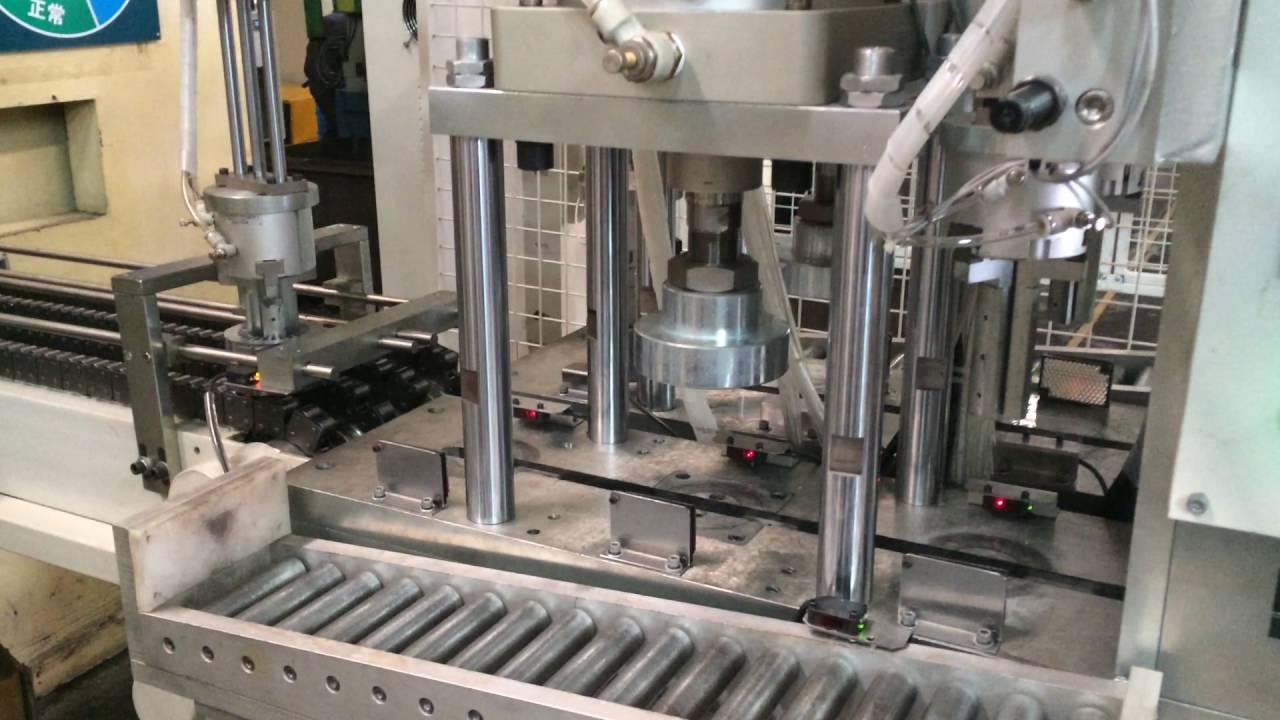
\includegraphics[height=0.6\textheight]{Figuras/Ch09/fig3}
\end{frame}


\begin{frame}{Funcionamento}
	\begin{block}{Tipos de tarefas}
		\begin{itemize}
			\item Um dispositivo de controle de qualidade deve remover produtos defeituosos (erros) \textbf{toda vez que ocorrerem} -- \textit{tarefa de evento}.
		\end{itemize}
	\end{block}
	
	\centering
	
	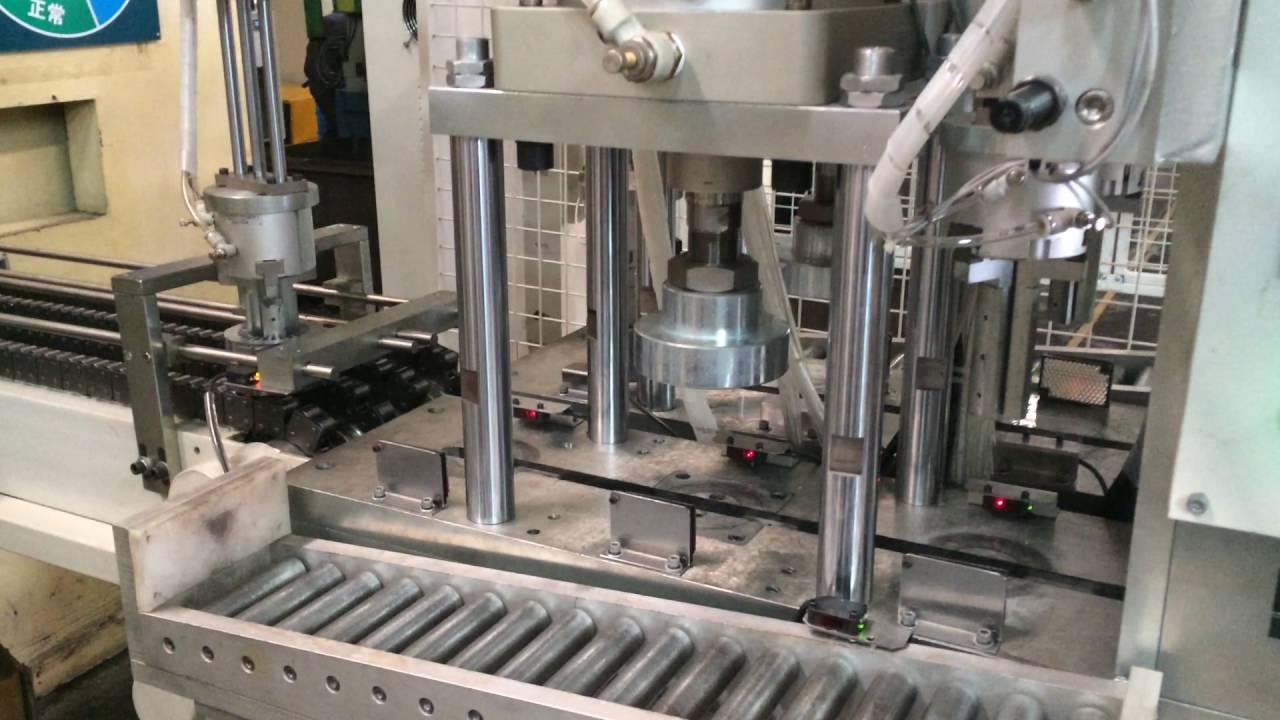
\includegraphics[height=0.6\textheight]{Figuras/Ch09/fig3}
\end{frame}


\begin{frame}{Funcionamento}
	\begin{block}{Prioridade de cada tarefa}
		As tarefas rodam no CLP com \textbf{diferentes prioridades}:
		\begin{itemize}
			\item As \textbf{tarefas de evento} tem a \textbf{maior prioridade}, já que devem lidar com \textbf{situações específicas}.
			\item As \textbf{tarefas de tempo} tem a \textbf{segunda maior} prioridade, já que devem ser executadas em \textbf{intervalos regulares}.
			\item Cada programa só pode ter \textbf{uma} tarefa contínua, que tem a \textbf{menor prioridade}.
		\end{itemize}
		Para certificar que o programa esteja rodando \textbf{normalmente}, existe uma função chamada \textit{Watch Dog Timer} (Temporizador de Cão de Guarda), que deve monitorar o \textbf{tempo de execução de cada tarefa} e \textbf{parar o CLP} caso passe de um \textbf{tempo estimado}.
		
		\medskip
		
		\textbf{Obs.:} É possível distinguir a prioridade entre duas ou mais tarefas de tempo ou de evento no mesmo programa.
	\end{block}
\end{frame}


\begin{frame}{Funcionamento}
	\centering
	
	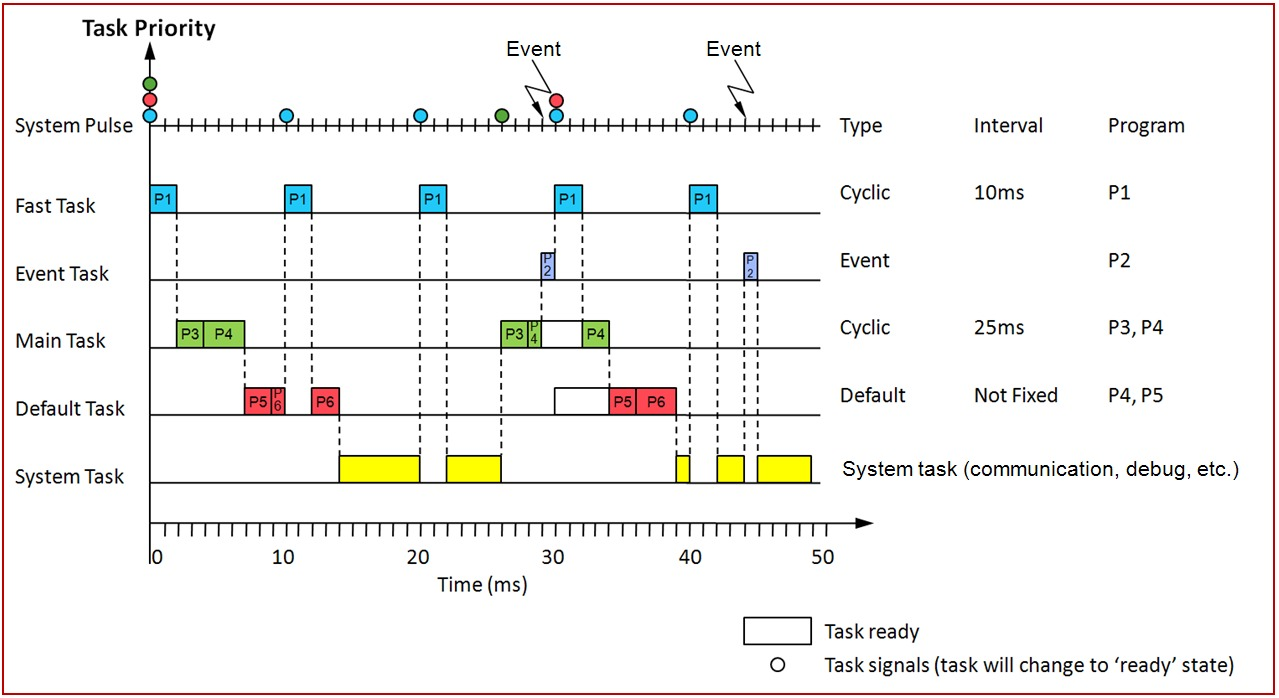
\includegraphics[height=0.8\textheight]{Figuras/Ch09/fig4}
	
	Prioridade de cada tarefa
\end{frame}


\begin{frame}{Funcionamento}
	\begin{block}{Estruturação de um projeto}
		Os projetos de CLP devem ser \textbf{bem organizados} para que, em trabalhos futuros, possamos \textbf{reutilizar} partes de projetos anteriores \textbf{sem problemas}.
		
		\smallskip
		
		Essa organização se dá em:
		\begin{itemize}
			\item Tarefas.
			\item Programas.
			\item Rotinas.
			\item Sub-rotinas.
		\end{itemize}
	\end{block}
\end{frame}


\begin{frame}{Funcionamento}
	\centering
	
	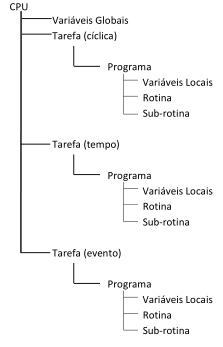
\includegraphics[height=0.8\textheight]{Figuras/Ch09/fig5}
	
	Estruturação de um projeto de CLP
\end{frame}


\begin{frame}{Funcionamento}
	\begin{block}{Estruturação de um projeto}
		\begin{itemize}
			\item As \textbf{tarefas} ditam o \textbf{comportamento} dos programas que se encontram dentro delas.
			\item Os \textbf{programas} são as \textbf{unidades funcionais} do projeto, que devem \textbf{executar funções macro específicas}.
			\item As \textbf{rotinas} devem \textbf{coordenar o funcionamento} de um programa.
			\item As \textbf{sub-rotinas} devem conter \textbf{instruções lógicas} para a execução de \textbf{pequenas tarefas}, de forma a \textbf{minimizar risco de falhas}.
		\end{itemize}
	\end{block}
\end{frame}


\begin{frame}{Funcionamento}
	\begin{block}{Estruturação de um projeto}
		As \textbf{variáveis} são responsáveis por \textbf{segurar dados} dentro de um projeto.
		
		\medskip
		
		A fim de facilitar ainda mais a organização, existem \textbf{dois tipos} de variáveis dentro de um projeto:
		\begin{itemize}
			\item Variáveis \textbf{globais}, que devem representar \textbf{objetos físicos} no projeto.
			\item Variáveis \textbf{locais}, que devem ser usadas como \textbf{suporte dentro de cada programa específico}.
		\end{itemize}
	\end{block}
\end{frame}


\frame{
	\frametitle{Exercícios}
	\begin{block}{}
		01. João é um colega que quer fazer um programa de CLP, mas não sabe por onde começar. Qual a sua sugestão para ele?
		
		\vspace{0.5cm}
		
		02. Sabendo que um CLP está em estado de \textbf{falha}, qual seria sua primeira preocupação?
		
		\vspace{0.5cm}
		
		03. Qual cartão deve ser usado para comandar uma \textbf{bomba hidráulica} via CLP? Por quê?
	\end{block}
}

\section*{Referências}
\frame{
	\frametitle{Referências e Exercícios Complementares}
	\begin{itemize}
		\item FRANCHI, Claiton Moro; CAMARGO, Valter Luis Arlindo de. Controladores Lógicos Programáveis - Sistemas Discretos, 1 ed. Érica, 2008.
		\item TAVARES, Leonardo; MONTEIRO, Natália Nogueira. Controladores Lógicos Programáveis, 1 ed. [s.n.], 2017.
	\end{itemize}
	%\centering{\alert{Página 546 - \textbf{Capítulo 6}}} \\
	%\centering{\alert{Lista de exercícios 01}}
}